%\chapter{About Figures}
%\label{chap-AboutFigures}
%\newthought{Figures in this chapter} are divided into two sections: 
%(1) figures from Tufte,
%(2) figures from other sources.
%

\section{Figures from Other Sources}
\label{chap-AboutFigures-Other}

\newthought{The file} {\tt fg-R-labs-wide-4-figures.tex}  
renders Figure~\ref{fg-R-labs-wide-4-figures}, used 
in\cite[27ex]{Lib-OPUS2-labs-2015-arxiv-Boskovic}.
\lipsum[1]
\begin{figure*}[t!]\index{Figures in R!4 panes}
% http://en.wikibooks.org/wiki/LaTeX/Floats,_Figures_and_Captions
% http://tex.stackexchange.com/questions/119984/subfigures-side-by-side-with-captions
%\usepackage{caption}     %% loads OK, but not needed neither subfigure nor subcaption
                          %% work under Tufte-book template
%\usepackage{subfigure}   %% This package loads without errors, however 
                          %% \begin{subfigure}[t]{0.49\textwidth} DOES NOT WORK!
%\usepackage{subcaption}  %% ! Package caption Error: The `subcaption' package does not work 
                          %%   correctly in compatibility mode.
\centering
\vspace*{-5ex}% removes white space at the top

\begin{minipage}{0.49\textwidth}
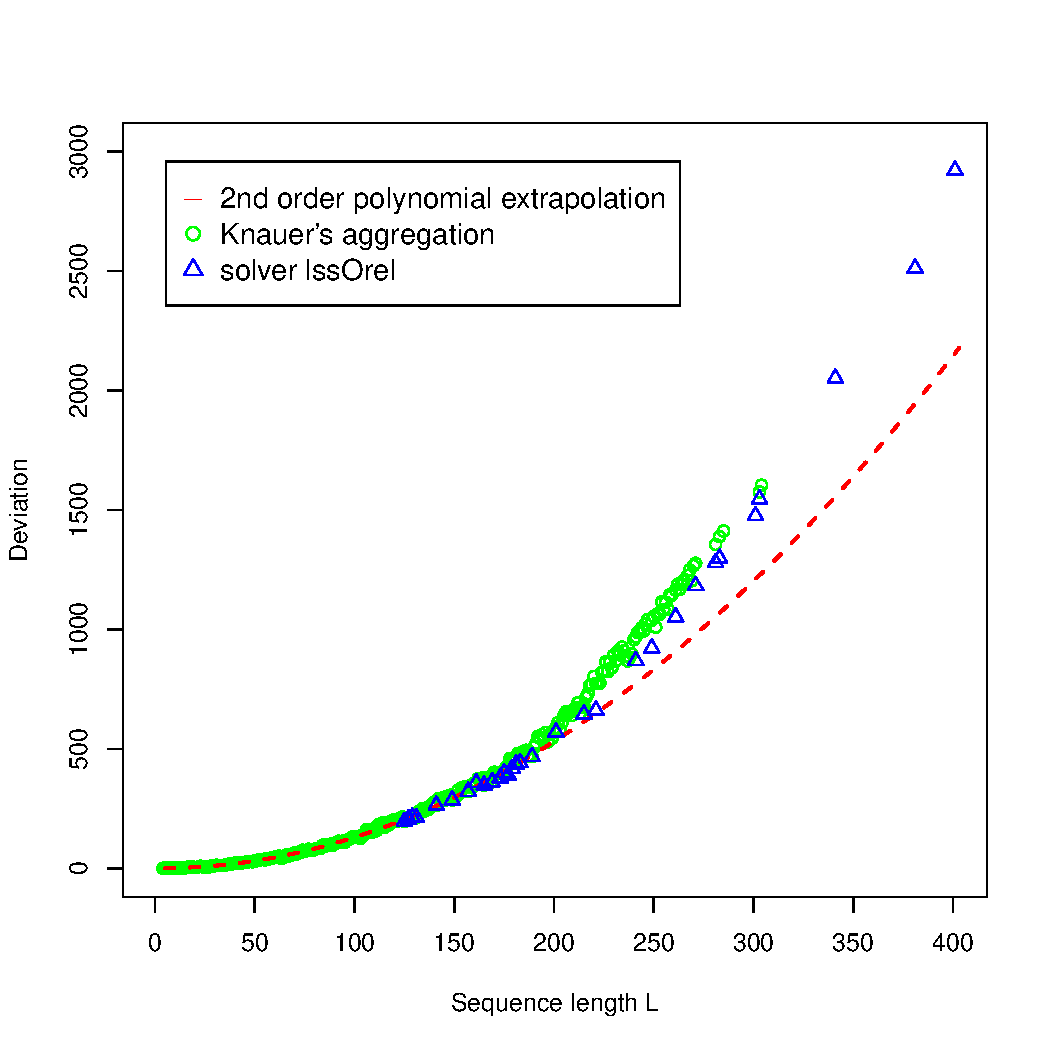
\includegraphics[width=0.99\textwidth]{fg-R-labs-wide-4-figures-a}
\vspace*{-5ex}% removes white space for the next row of figures
\end{minipage}
\begin{minipage}{0.49\textwidth}
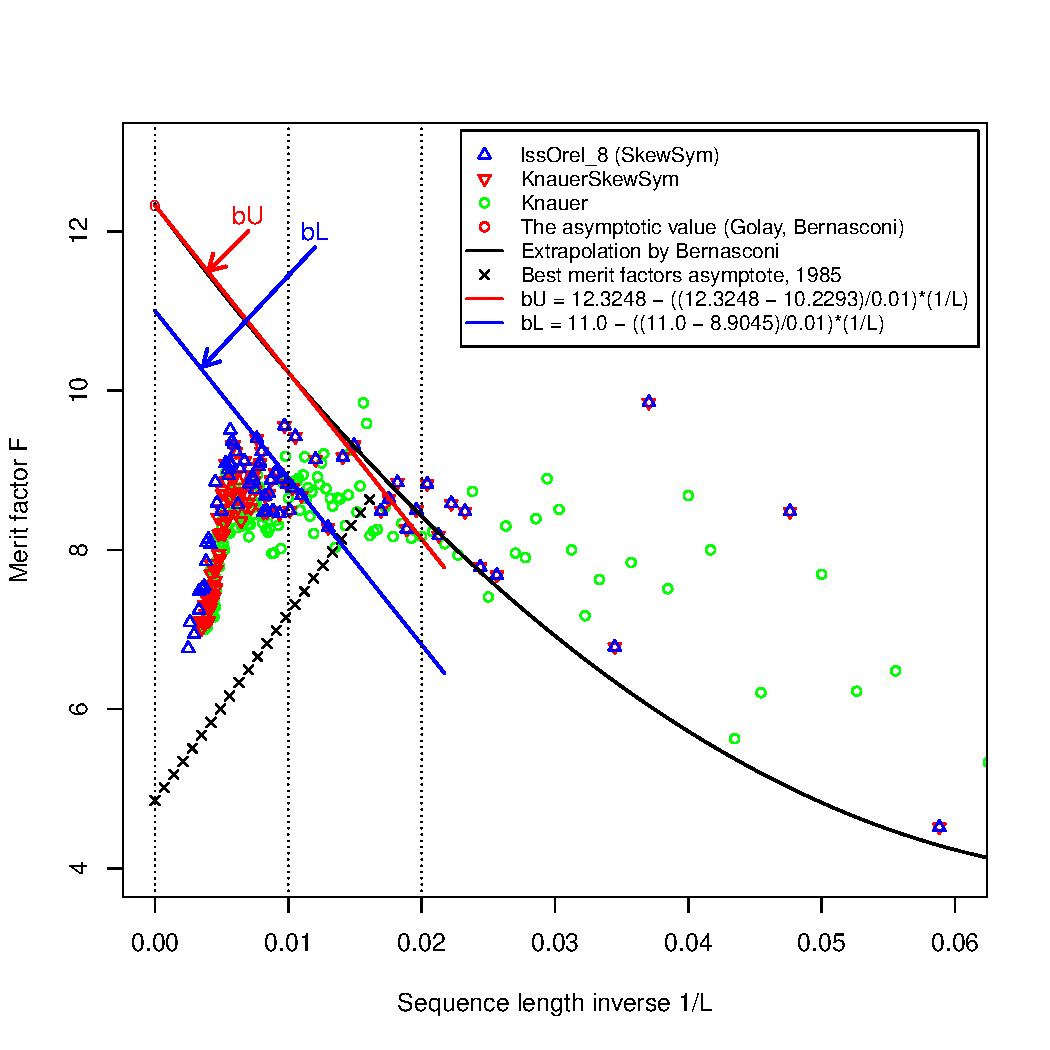
\includegraphics[width=0.99\textwidth]{fg-R-labs-wide-4-figures-b}
\vspace*{-5ex}% removes white space for the next row of figures
\end{minipage}
~%
\begin{minipage}{0.49\textwidth}
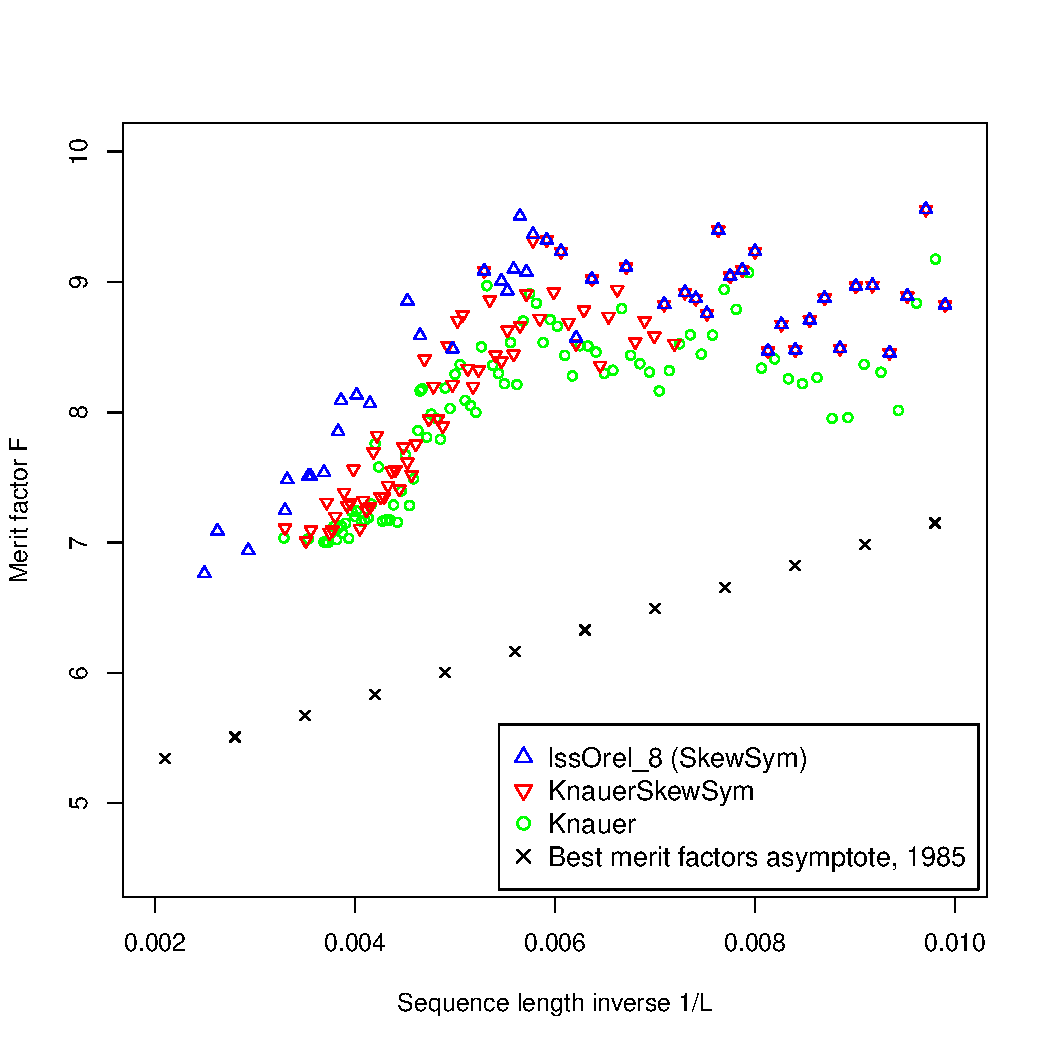
\includegraphics[width=0.99\textwidth]{fg-R-labs-wide-4-figures-c}
%\vspace*{-1ex}
\end{minipage}
%
\begin{minipage}{0.49\textwidth}
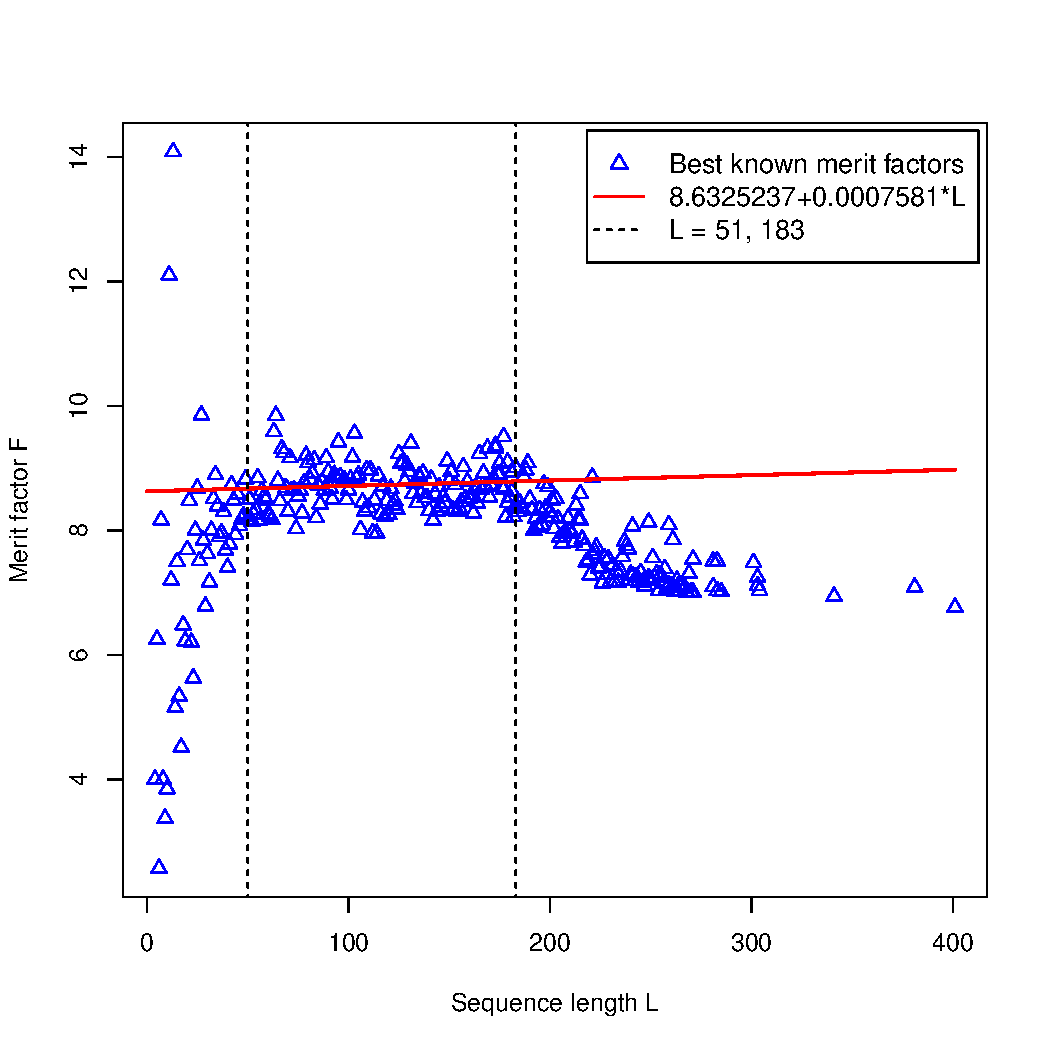
\includegraphics[width=0.99\textwidth]{fg-R-labs-wide-4-figures-d}
%\vspace*{-1ex}
\end{minipage}
%
\caption[From the file fg-R-labs-wide-4-figures.tex][3ex]
{From the file fg-R-labs-wide-4-figures.tex {\em borrowed from} {\tt Lib-OPUS2-labs-2015-arxiv-Boskovic}. 
{\bf NOTE: both `verb' and `cite' commands seem disabled under `figure environment'!}
(a) 
it may not be possible to create (a) in this file with \LaTeX ... may need to create it in R;
%
(b)
it may not be possible to create (b) in this file with \LaTeX ... may need to create it in R;
%
(c)
it may not be possible to create (c) in this file with \LaTeX ... may need to create it in R;
%
(d) 
it may not be possible to create (d) in this file with \LaTeX ... may need to create it in R.
}
\label{fg-R-labs-wide-4-figures}
\end{figure*}



\begin{figure*}[t!]\index{Figures in R!6 panes}
% http://en.wikibooks.org/wiki/LaTeX/Floats,_Figures_and_Captions
% http://tex.stackexchange.com/questions/119984/subfigures-side-by-side-with-captions
%\usepackage{caption}     %% loads OK, but not needed neither subfigure nor subcaption
                          %% work under Tufte-book template
%\usepackage{subfigure}   %% This package loads without errors, however 
                          %% \begin{subfigure}[t]{0.49\textwidth} DOES NOT WORK!
%\usepackage{subcaption}  %% ! Package caption Error: The `subcaption' package does not work 
                          %%   correctly in compatibility mode.
\centering
\vspace*{-5ex}% removes white space at the top

\begin{minipage}{0.49\textwidth}
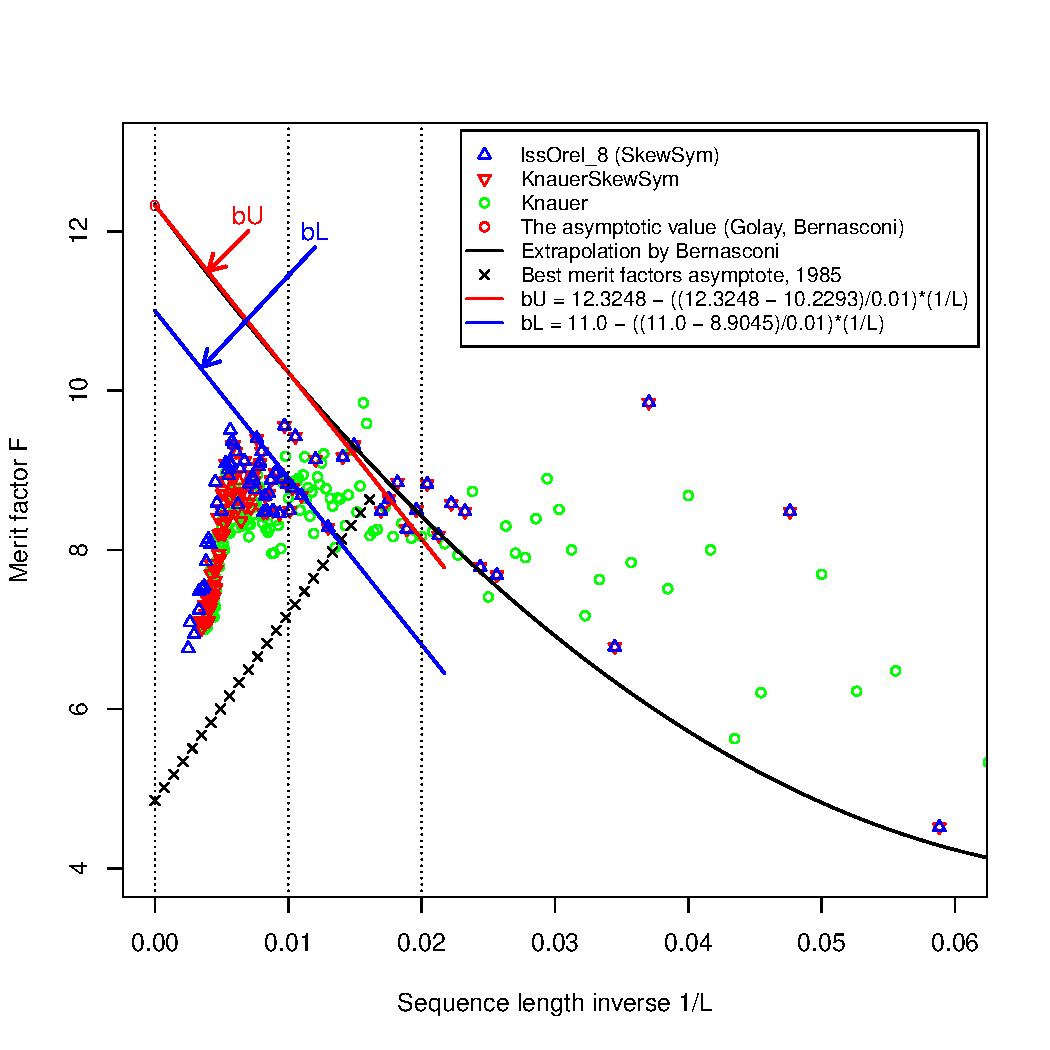
\includegraphics[width=0.99\textwidth]{fg-R-labs-wide-4-figures-b}
\vspace*{-5ex}% removes white space for the next row of figures
\end{minipage}
\begin{minipage}{0.49\textwidth}
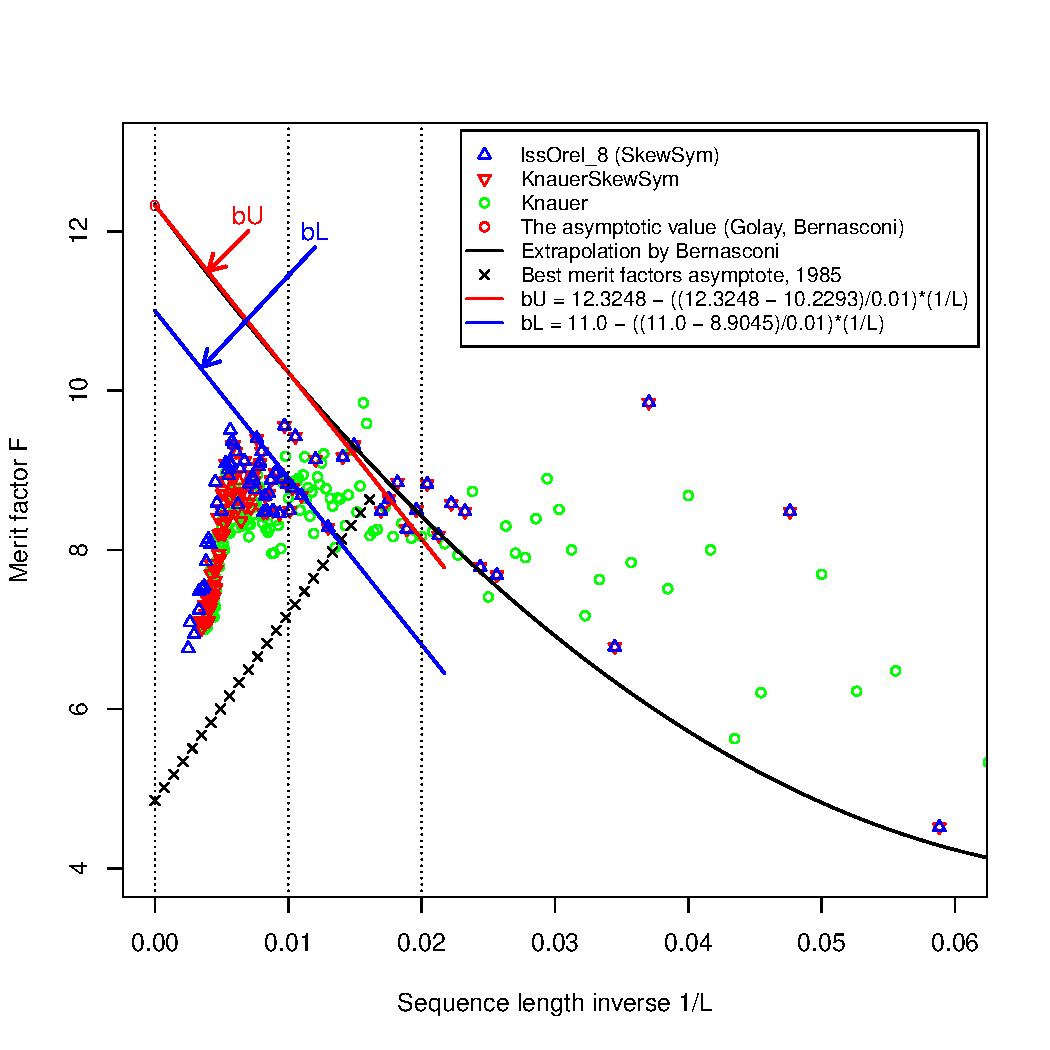
\includegraphics[width=0.99\textwidth]{fg-R-labs-wide-4-figures-b}
\vspace*{-5ex}% removes white space for the next row of figures
\end{minipage}
~%
\begin{minipage}{0.49\textwidth}
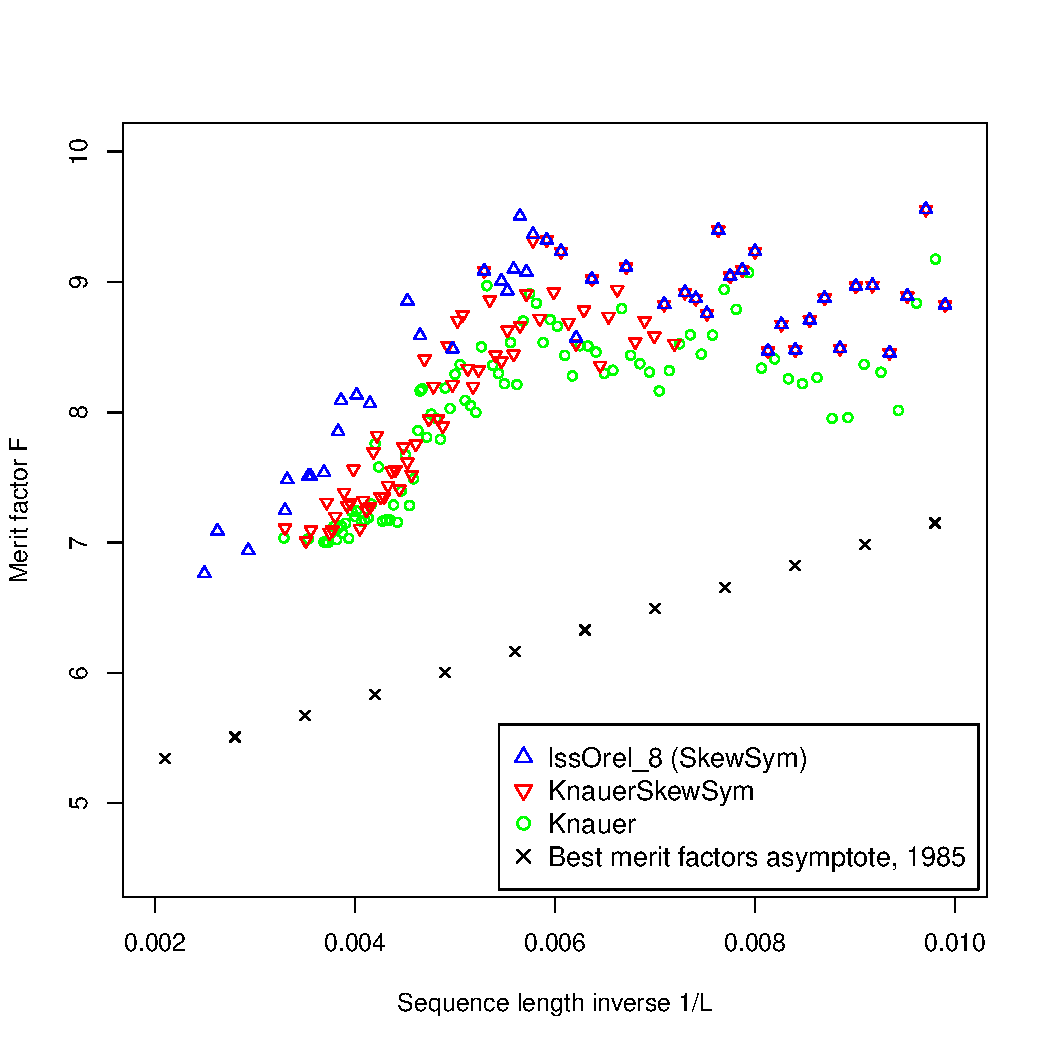
\includegraphics[width=0.99\textwidth]{fg-R-labs-wide-4-figures-c}
\vspace*{-5ex}% removes white space for the next row of figures
\end{minipage}
%
\begin{minipage}{0.49\textwidth}
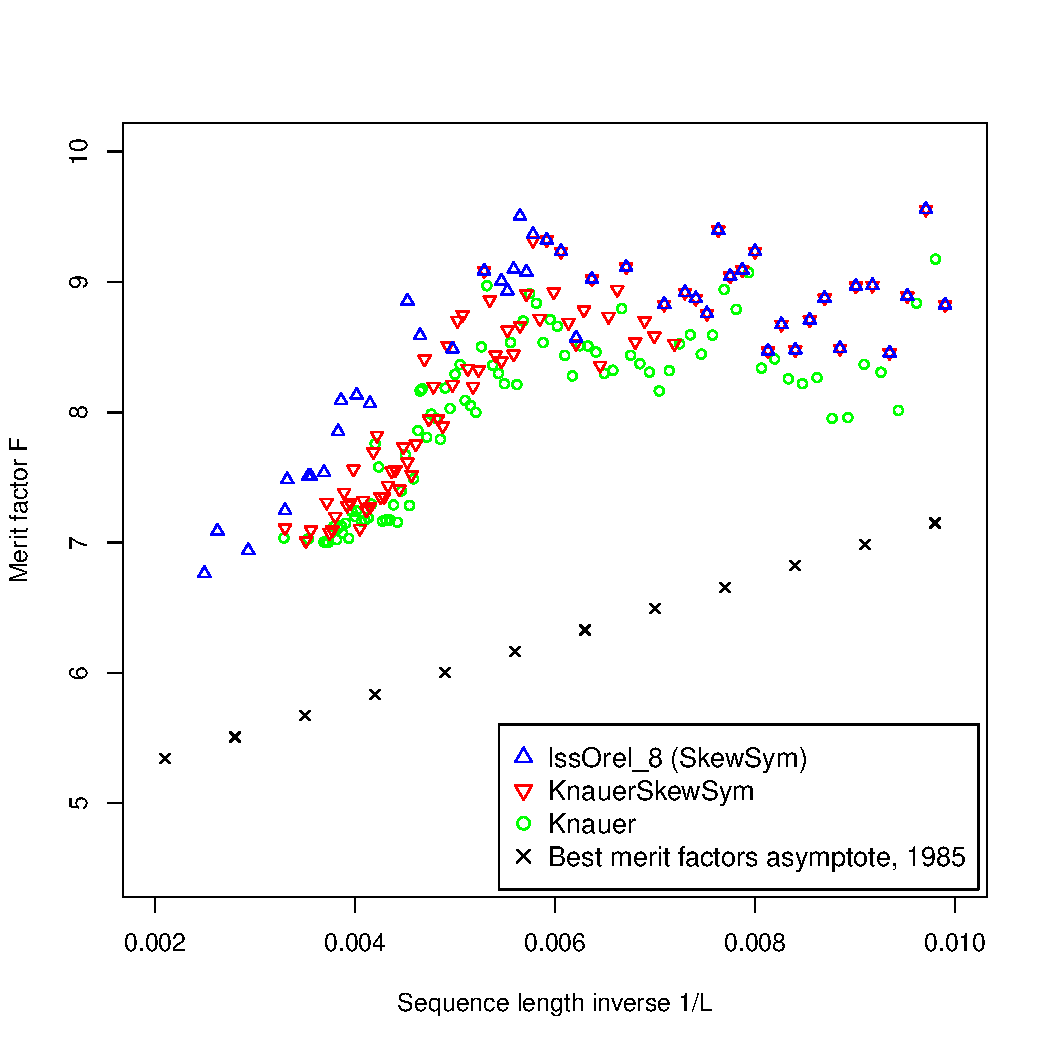
\includegraphics[width=0.99\textwidth]{fg-R-labs-wide-4-figures-c}
\vspace*{-5ex}% removes white space for the next row of figures
\end{minipage}
~%
\begin{minipage}{0.49\textwidth}
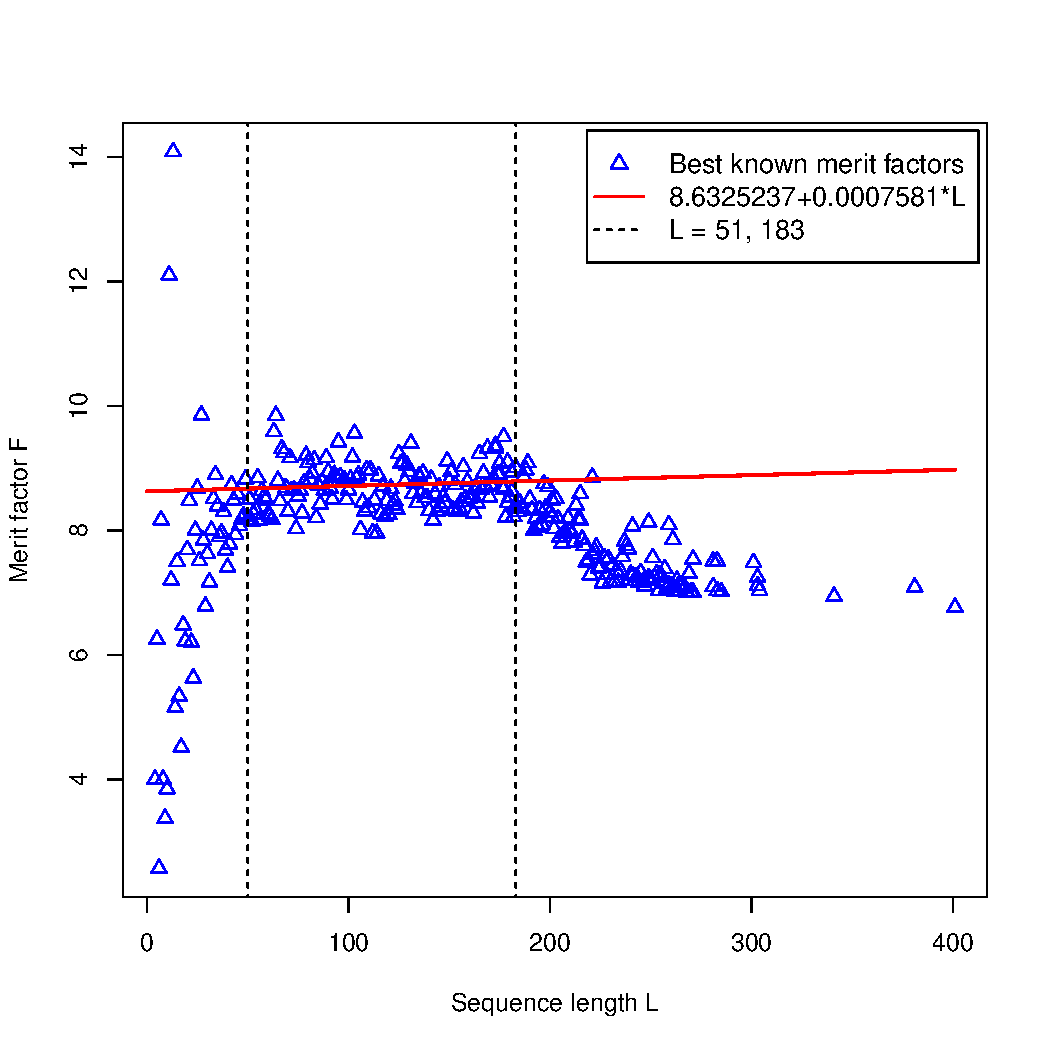
\includegraphics[width=0.99\textwidth]{fg-R-labs-wide-4-figures-d}
%\vspace*{-1ex}
\end{minipage}
%
\begin{minipage}{0.49\textwidth}
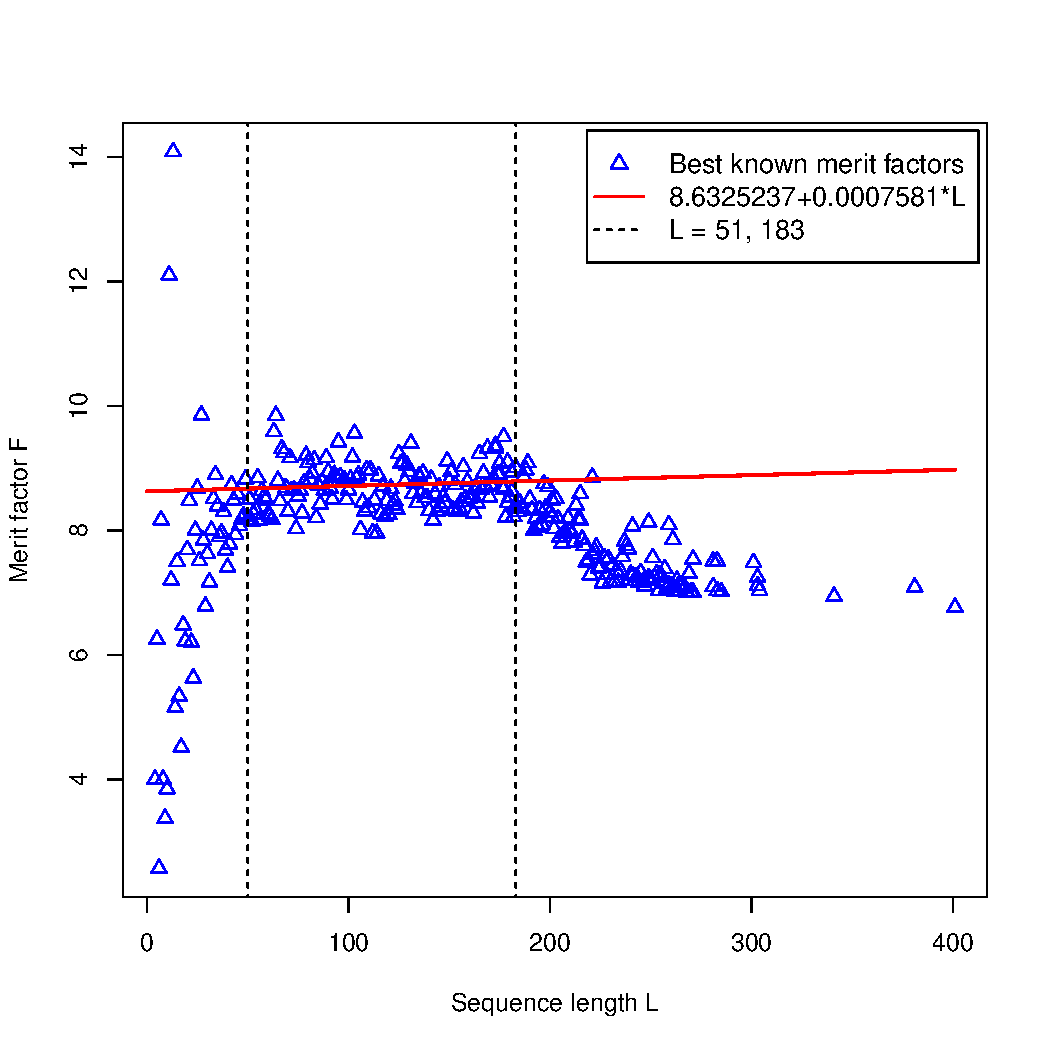
\includegraphics[width=0.99\textwidth]{fg-R-labs-wide-4-figures-d}
%\vspace*{-1ex}
\end{minipage}
%
\caption[From the file fg-R-labs-wide-6-figures.tex]
{From the file fg-R-labs-wide-6-figures.tex {\em borrowed from} {\tt Lib-OPUS2-labs-2015-arxiv-Boskovic}. 
}
\label{fg-R-labs-wide-6-figures}
\end{figure*}




\newthought{The file}  {\tt fg-R-labs-wide-6-figures.tex}  
renders Figure~\ref{fg-R-labs-wide-6-figures}.
\lipsum[1]
\clearpage

\begin{figure}[t!]
% http://en.wikibooks.org/wiki/LaTeX/Floats,_Figures_and_Captions
% http://tex.stackexchange.com/questions/119984/subfigures-side-by-side-with-captions
%\usepackage{caption}     %% loads OK, but not needed neither subfigure nor subcaption
                          %% work under Tufte-book template
%\usepackage{subfigure}   %% This package loads without errors, however 
                          %% \begin{subfigure}[t]{0.49\textwidth} DOES NOT WORK!
%\usepackage{subcaption}  %% ! Package caption Error: The `subcaption' package does not work 
                          %%   correctly in compatibility mode.
\centering
\vspace*{-5ex}% removes white space at the top

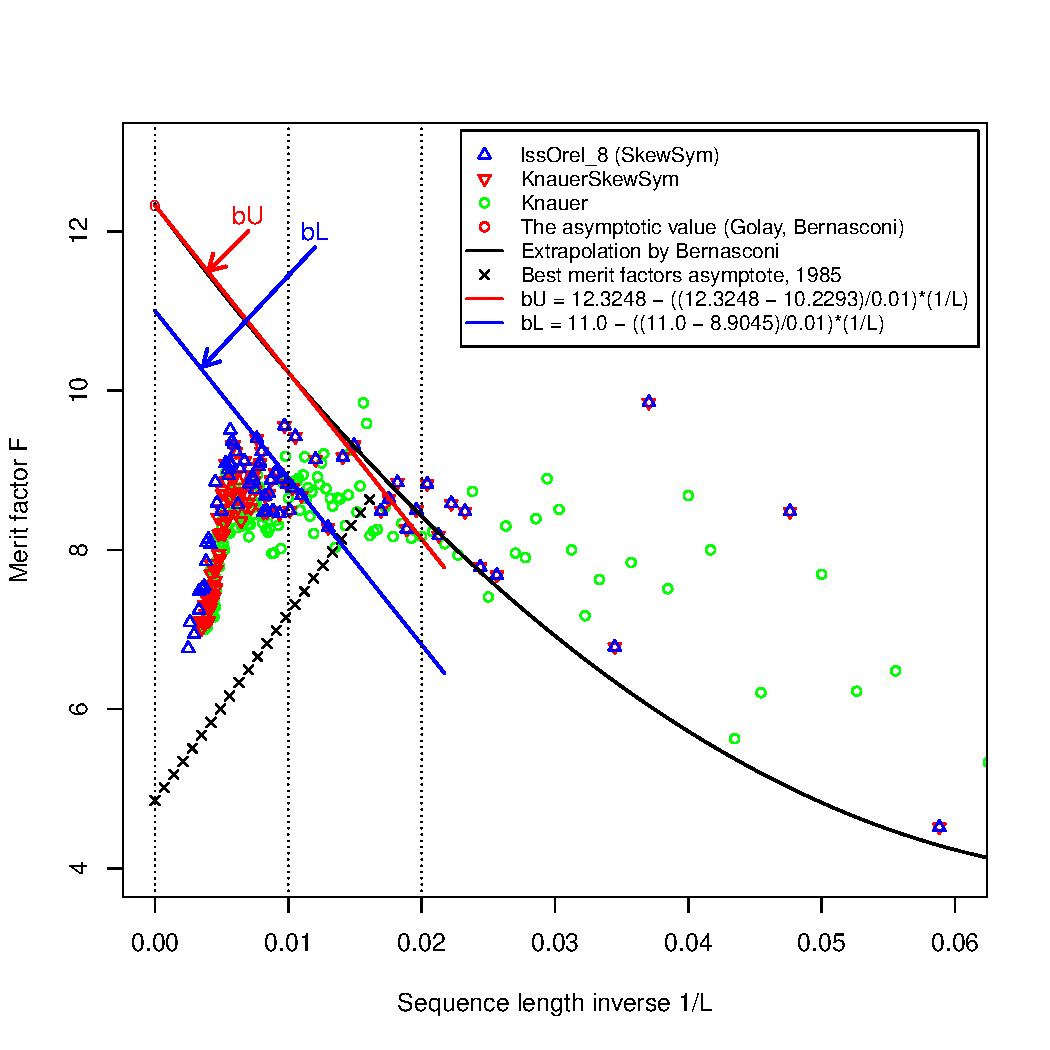
\includegraphics[width=0.79\textwidth]{fg-R-labs-wide-4-figures-b}
\vspace*{-5ex}% removes white space for the next figure 
\\
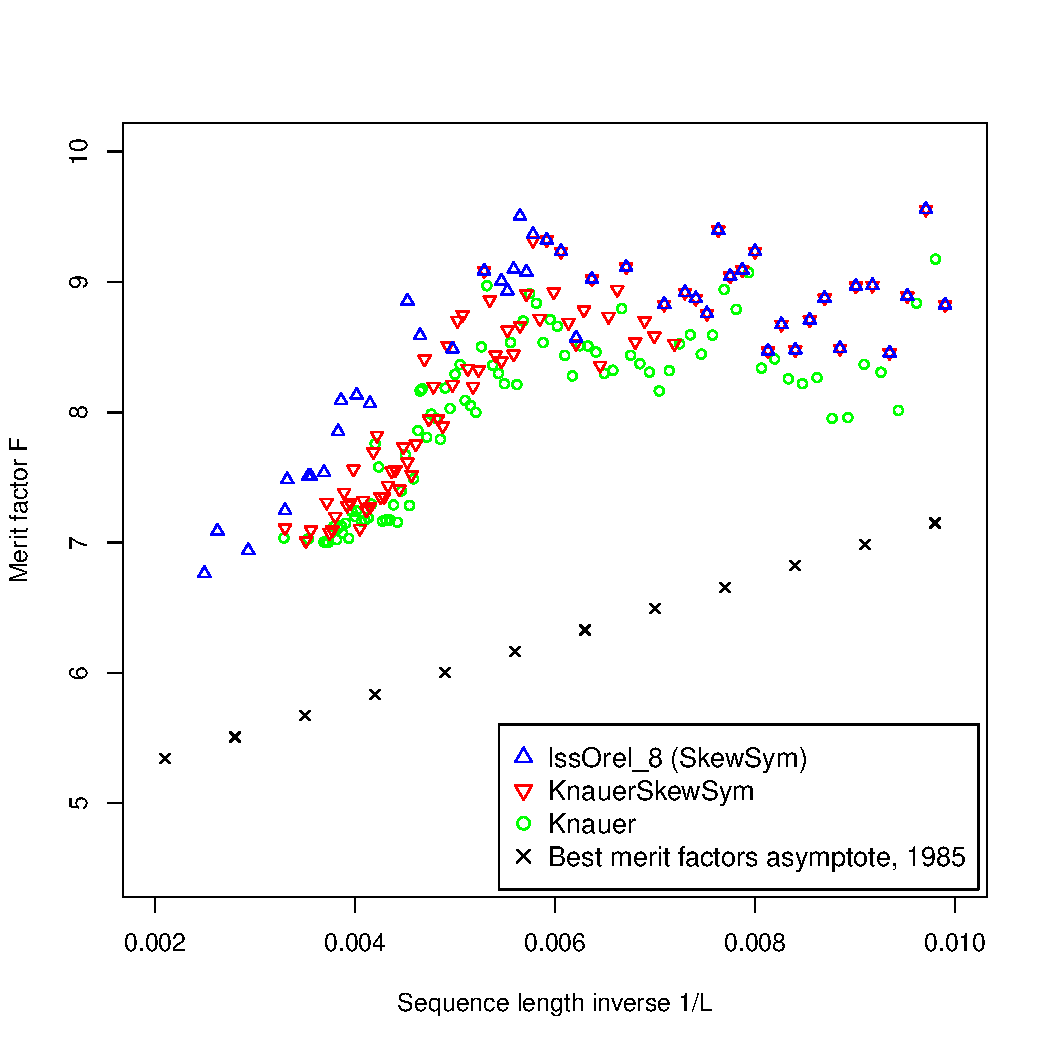
\includegraphics[width=0.79\textwidth]{fg-R-labs-wide-4-figures-c}
\vspace*{-5ex}% removes white space for the next figure 
\\
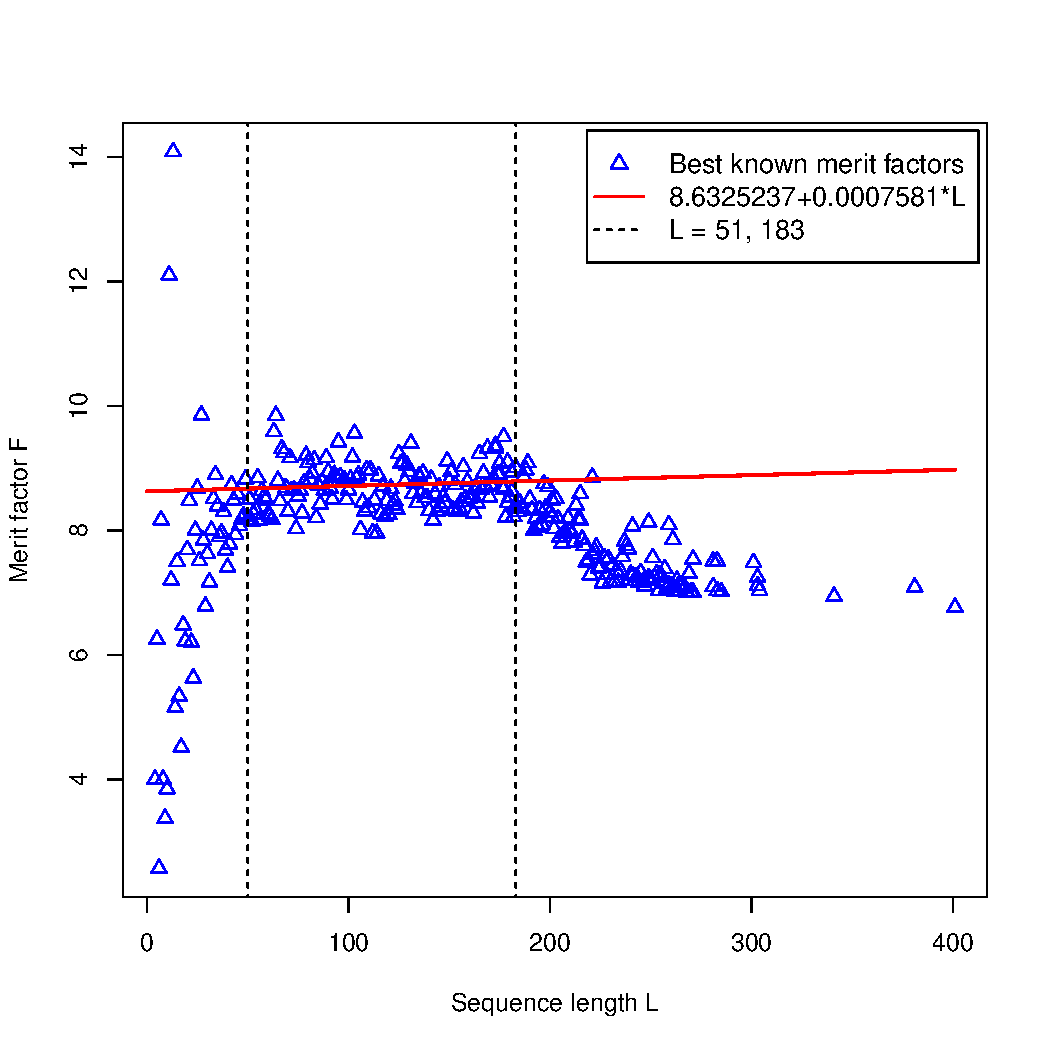
\includegraphics[width=0.79\textwidth]{fg-R-labs-wide-4-figures-d}
\vspace*{-5ex}% removes white space for the next figure 
%
\caption[From the file fg-R-labs-normal-3-figures.tex]
{From the file fg-R-labs-normal-3-figures.tex {\em borrowed from} {\tt Lib-OPUS2-labs-2015-arxiv-Boskovic}.
{\bf NOTE: both `verb' and `cite' commands seem disabled under `figure environment'!}
Also, 3 vertical plots in portrait from R create more white space than the 4 plots 
from R in wide format, see Figure~\ref{fg-R-labs-wide-4-figures}.
Then,
(a) 
it may not be possible to create (a) in this file with \LaTeX ... may need to create it in R;
%
(b)
it may not be possible to create (b) in this file with \LaTeX ... may need to create it in R;
%
(c)
it may not be possible to create (c) in this file with \LaTeX ... may need to create it in R.
}
\label{fg-R-labs-normal-3-figures}
\end{figure}



\newthought{The file}  {\tt fg-R-labs-normal-3-figures.tex}  
renders Figure~\ref{fg-R-labs-normal-3-figures}.
{\bf NOTE AGAIN: both `verb' and `cite' commands seem disabled under `figure environment'!}
\lipsum[2]

\begin{figure}[t!]
% http://en.wikibooks.org/wiki/LaTeX/Floats,_Figures_and_Captions
% http://tex.stackexchange.com/questions/119984/subfigures-side-by-side-with-captions
%\usepackage{caption}     %% loads OK, but not needed neither subfigure nor subcaption
                          %% work under Tufte-book template
%\usepackage{subfigure}   %% This package loads without errors, however 
                          %% \begin{subfigure}[t]{0.49\textwidth} DOES NOT WORK!
%\usepackage{subcaption}  %% ! Package caption Error: The `subcaption' package does not work 
                          %%   correctly in compatibility mode.
\centering
\vspace*{-0ex}% removes white space at the top

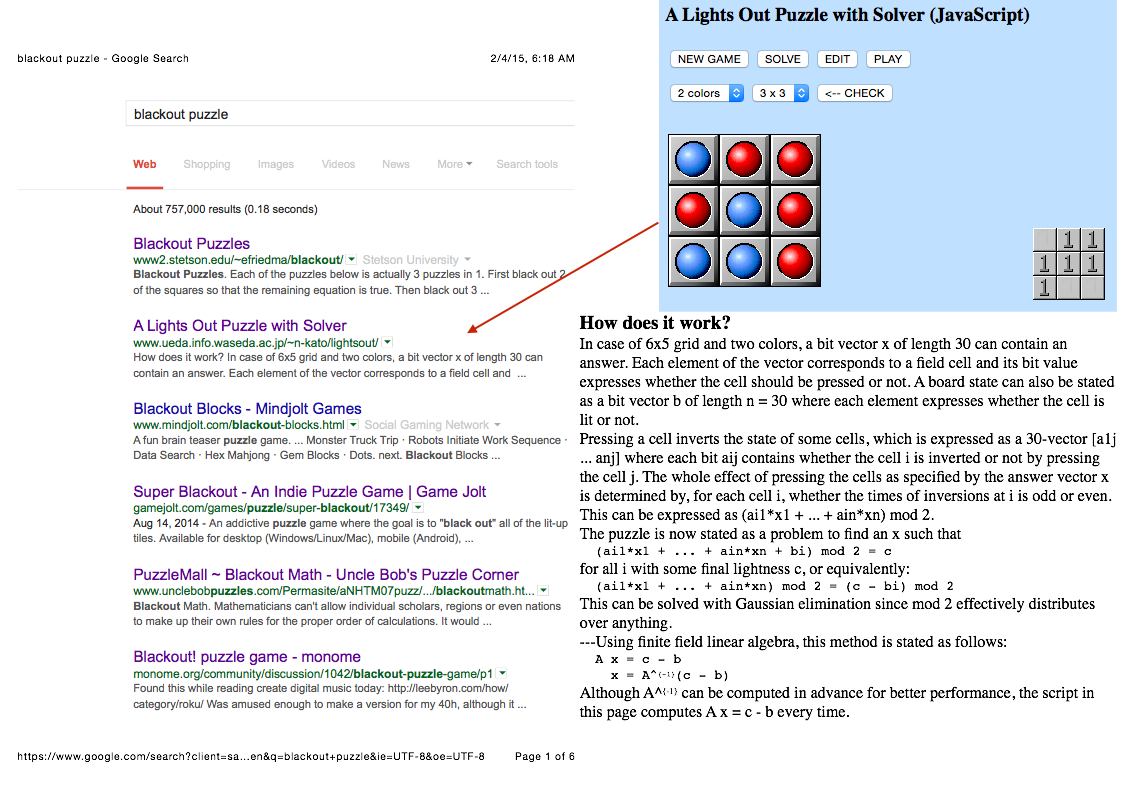
\includegraphics[width=0.99\textwidth]{fg-key-blackp-descr-a}
\vspace*{1ex}% removes white space for the next figure 
\\
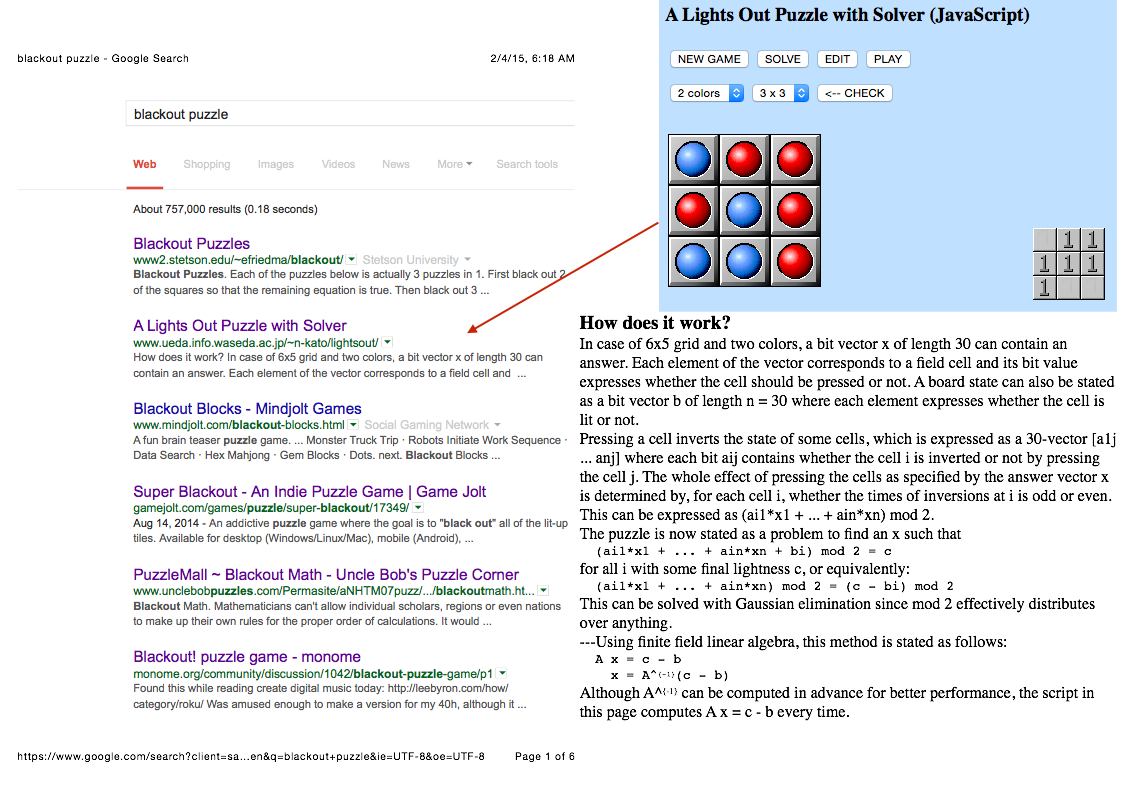
\includegraphics[width=0.99\textwidth]{fg-key-blackp-descr-a}
\vspace*{1ex}% removes white space for the next figure 
\\
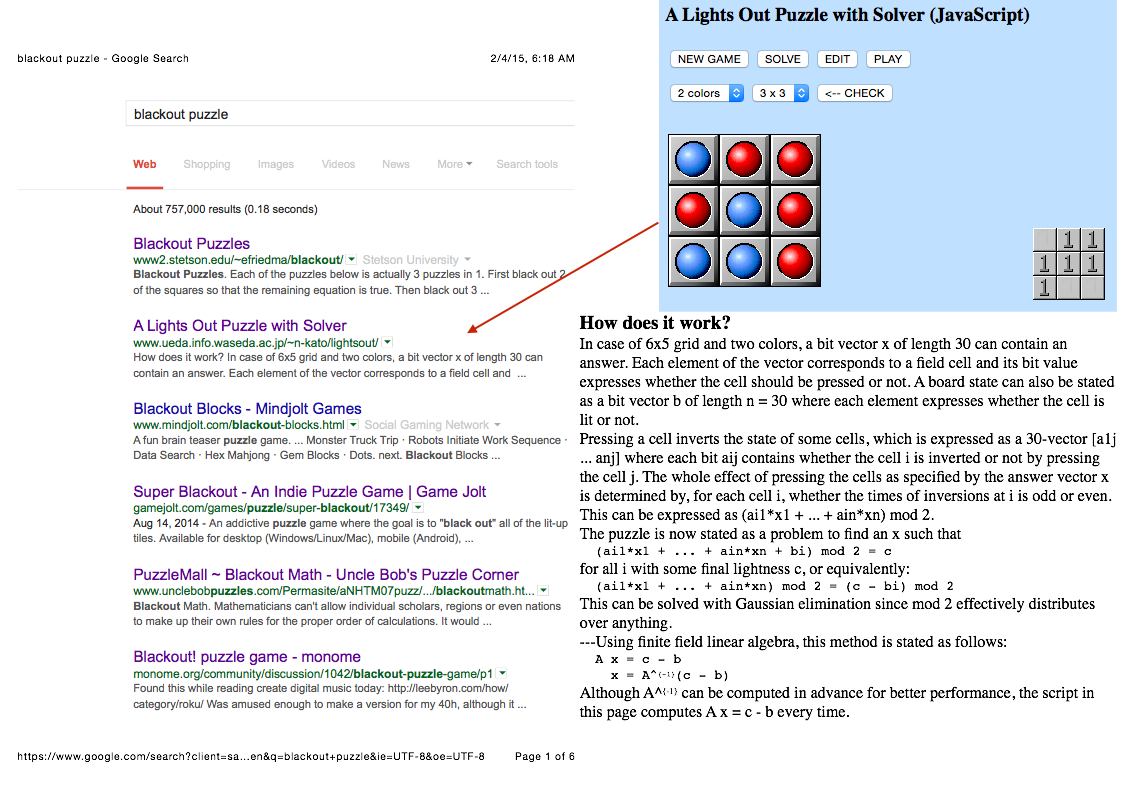
\includegraphics[width=0.99\textwidth]{fg-key-blackp-descr-a}
\vspace*{1ex}% removes white space for the next figure 
%
% https://github.com/fbrglez/gitPublic/tree/master/xProj499-Sp15
\caption[From the file fg-key-blackp-normal-3-figures.tex]
{From the file fg-key-blackp-portrait-3-figures.tex {\em borrowed from} {\tt Lib-OPUS2-ebook-CSC499-Sp15-2015-Brglez}.
{\bf NOTE: both `verb' and `cite' commands seem disabled under `figure environment'!}
Also, the portrait of 3 plots from Keynote are larger than the 3 plots from R in portrait format,
see Figure~\ref{fg-R-labs-portrait-3-figures}.
Then,
(a) 
it may not be possible to create (a) in this file with \LaTeX ... may need to create it in Keynote;
%
(b)
it may not be possible to create (b) in this file with \LaTeX ... may need to create it in Keynote;
%
(c)
it may not be possible to create (c) in this file with \LaTeX ... may need to create it in Keynote.
}
\label{fg-key-blackp-normal-3-figures}
\end{figure}



\newthought{The file}
fg-key-blackp-normal-3-figures, first used 
in\cite[27ex]{Lib-OPUS2-ebook-CSC499-Sp15-2015-Brglez},
renders Figure~\ref{fg-key-blackp-normal-3-figures}.
\lipsum[3]

\begin{figure}[h!]

\centering
\vspace*{-0ex}% removes white space at the top
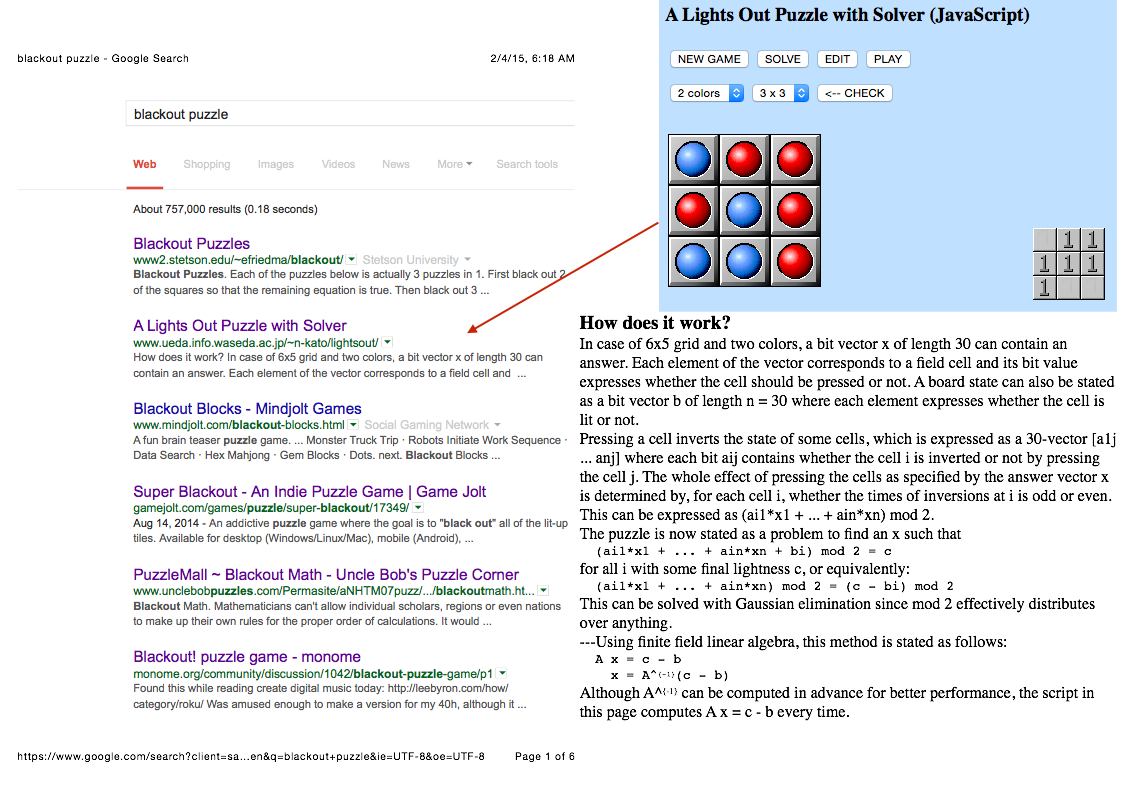
\includegraphics[width=0.85\textwidth]{fg-key-blackp-descr-a}

\caption[From the file fg-key-blackp-normal-1-figures.tex]
{From the file fg-key-blackp-normal-2-figures.tex {\em borrowed from} {\tt Lib-OPUS2-ebook-CSC499-Sp15-2015-Brglez}.
{\bf NOTE: both `verb' and `cite' commands seem disabled under `figure environment'!}
}
\label{fg-key-blackp-normal-1-figure}
\end{figure}



\begin{figure}[h!]

\centering
\vspace*{-0ex}% removes white space at the top
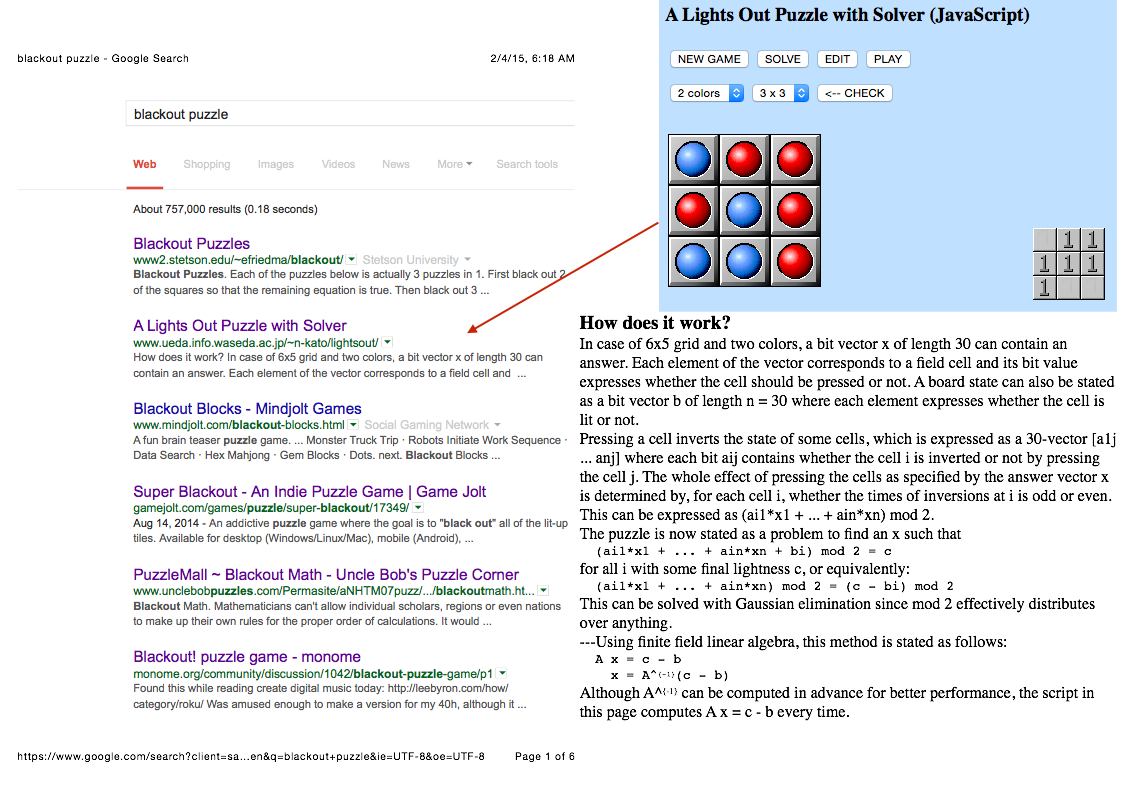
\includegraphics[width=0.85\textwidth]{fg-key-blackp-descr-a}

\caption[From the file fg-key-blackp-normal-1-figures.tex]
{From the file fg-key-blackp-normal-2-figures.tex {\em borrowed from} {\tt Lib-OPUS2-ebook-CSC499-Sp15-2015-Brglez}.
{\bf NOTE: both `verb' and `cite' commands seem disabled under `figure environment'!}
}
\label{fg-key-blackp-normal-1-figure}
\end{figure}



\begin{figure}[h!]

\centering
\vspace*{-0ex}% removes white space at the top
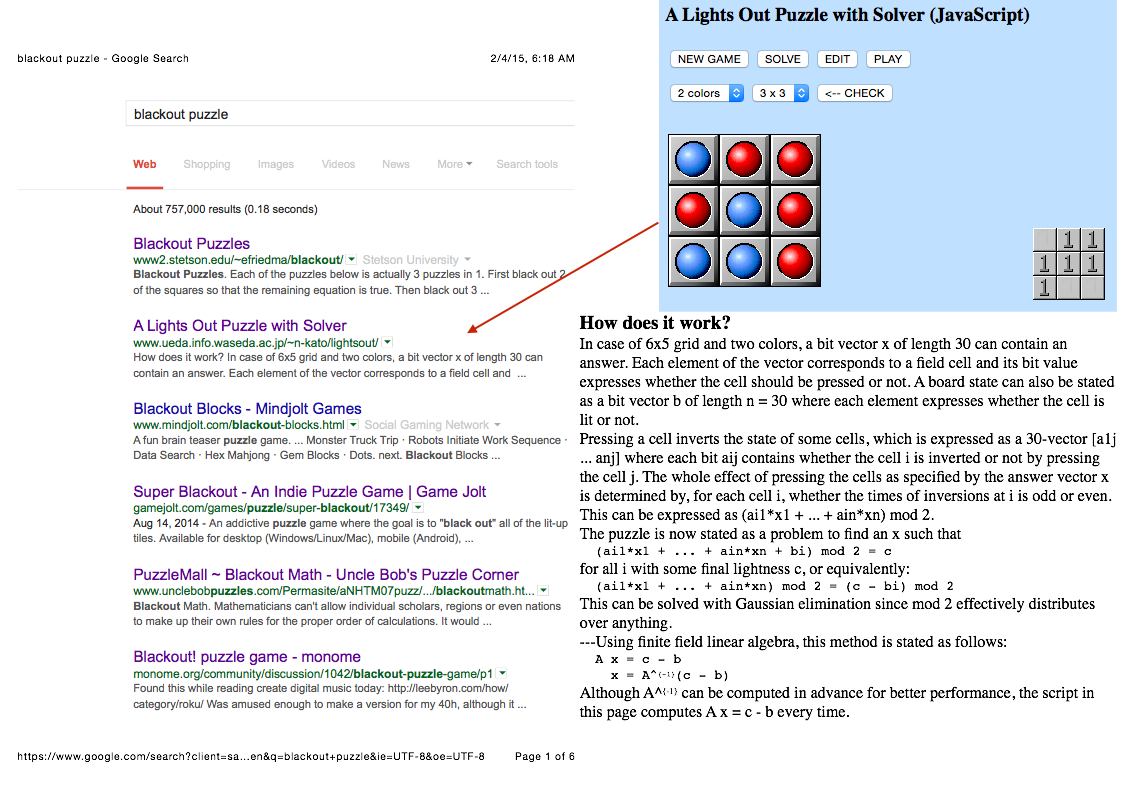
\includegraphics[width=0.85\textwidth]{fg-key-blackp-descr-a}

\caption[From the file fg-key-blackp-normal-1-figures.tex]
{From the file fg-key-blackp-normal-2-figures.tex {\em borrowed from} {\tt Lib-OPUS2-ebook-CSC499-Sp15-2015-Brglez}.
{\bf NOTE: both `verb' and `cite' commands seem disabled under `figure environment'!}
}
\label{fg-key-blackp-normal-1-figure}
\end{figure}




\newthought{The file}
fg-key-blackp-normal-1-figure.tex  
renders Figure~\ref{fg-key-blackp-normal-1-figure}.
\lipsum[4]
\lipsum[4]


\clearpage
\newthought{The file}
fg-key-blackp-wide-1-figure.tex, 
renders Figure~\ref{fg-key-blackp-wide-1-figure}.

\begin{figure*}[t!]

\centering
\vspace*{-0ex}% removes white space at the top
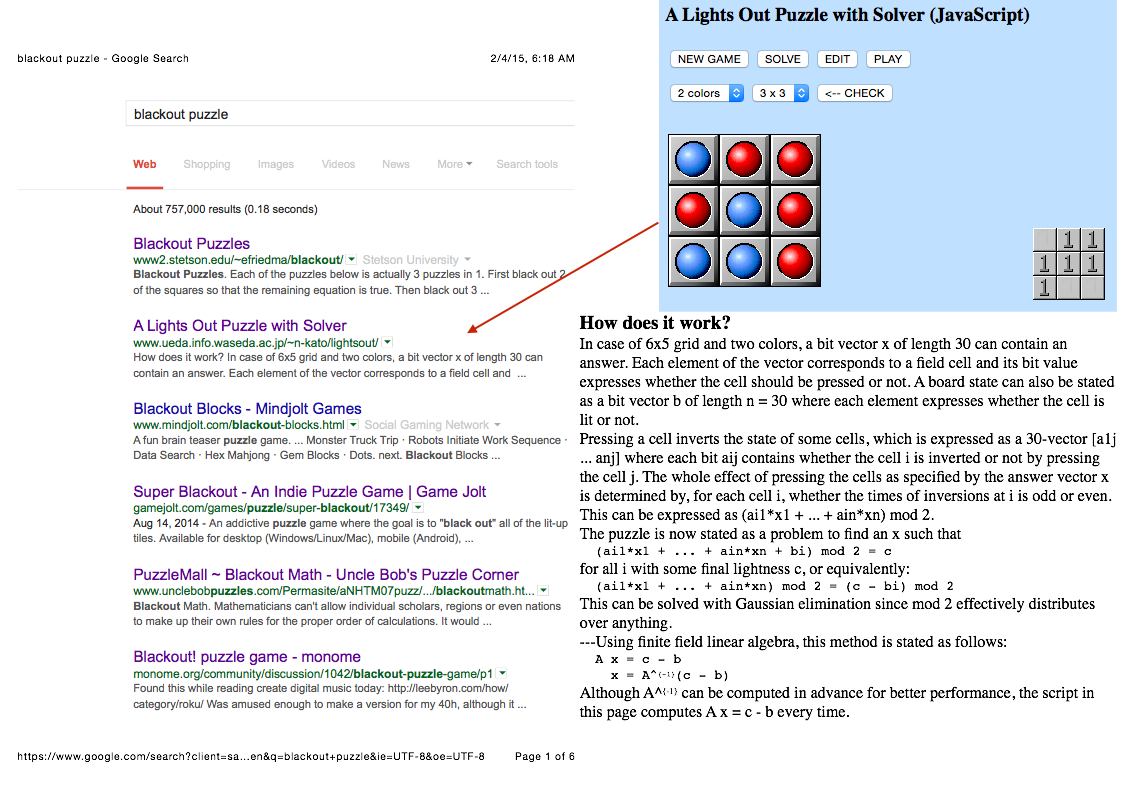
\includegraphics{fg-key-blackp-descr-a}

\caption[From the file fg-key-blackp-wide-1-figures.tex]
{From the file fg-key-blackp-wide-1-figures.tex {\em borrowed from} {\tt Lib-OPUS2-ebook-CSC499-Sp15-2015-Brglez}.
}
\label{fg-key-blackp-wide-1-figure}
\end{figure*}




\lipsum[4]
\begin{figure*}[t!]

\centering
\vspace*{-0ex}% removes white space at the top
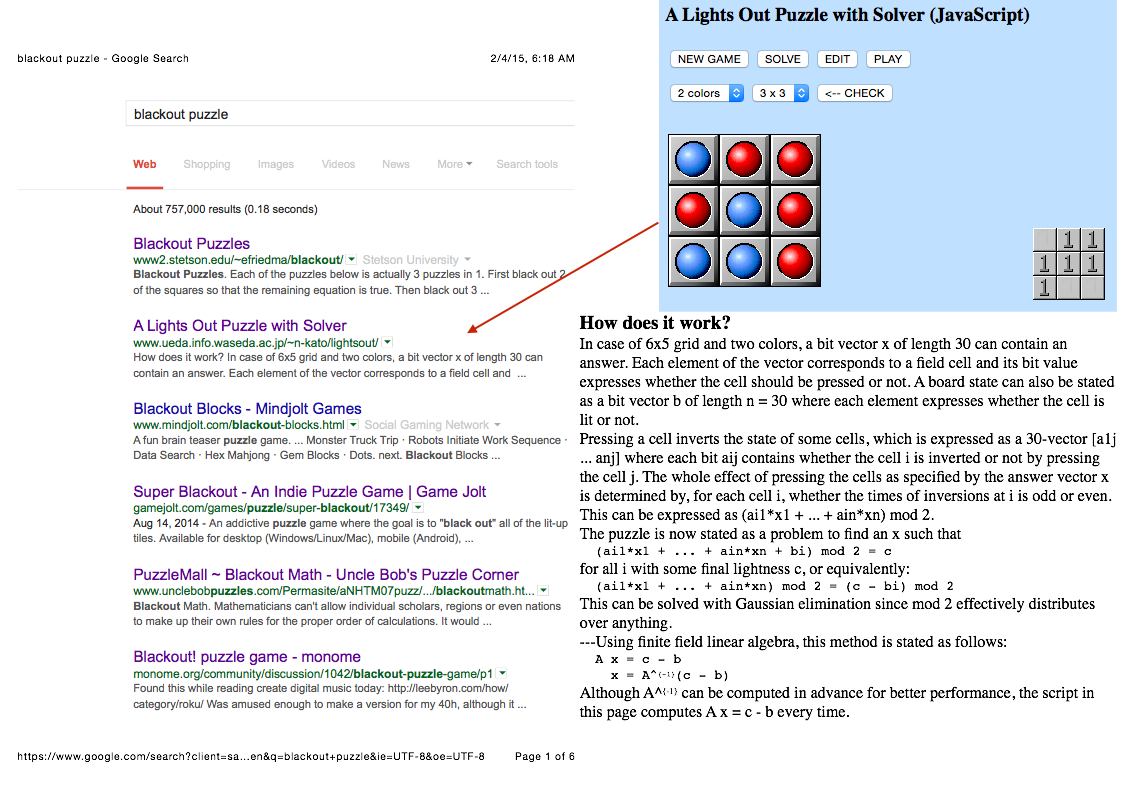
\includegraphics[width=0.90\textwidth]{fg-key-blackp-descr-a}
\\[3ex]
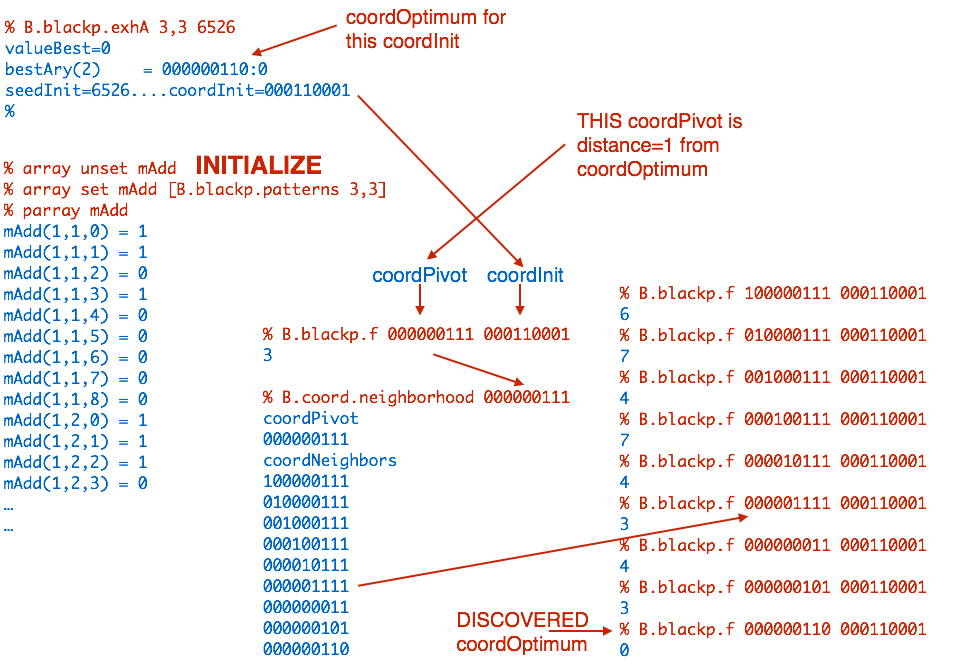
\includegraphics[width=0.90\textwidth]{fg-key-blackp-neighbors}

\caption[From the file fg-key-blackp-wide-2-figures.tex]
{From the file fg-key-blackp-wide-2-figures.tex {\em borrowed from} {\tt Lib-OPUS2-ebook-CSC499-Sp15-2015-Brglez}.
}
\label{fg-key-blackp-wide-2-figures}
\end{figure*}



\newthought{The file}
fg-key-blackp-wide-2-figures.tex  
renders Figure~\ref{fg-key-blackp-wide-2-figures}.
The file
fg-key-blackp-wide-2-figures.tex  
renders Figure~\ref{fg-key-blackp-wide-2-figures}.
The file
fg-key-blackp-wide-2-figures.tex  
renders Figure~\ref{fg-key-blackp-wide-2-figures}.
The file
fg-key-blackp-wide-2-figures.tex  
renders Figure~\ref{fg-key-blackp-wide-2-figures}.
The file
fg-key-blackp-wide-2-figures.tex  
renders Figure~\ref{fg-key-blackp-wide-2-figures}.
The file
fg-key-blackp-wide-2-figures.tex  
renders Figure~\ref{fg-key-blackp-wide-2-figures}.
The file
fg-key-blackp-wide-2-figures.tex  
renders Figure~\ref{fg-key-blackp-wide-2-figures}.

\clearpage
\begin{figure*}[t!]

\centering
\vspace*{-5ex}% removes white space at the top

\begin{minipage}{0.49\textwidth}
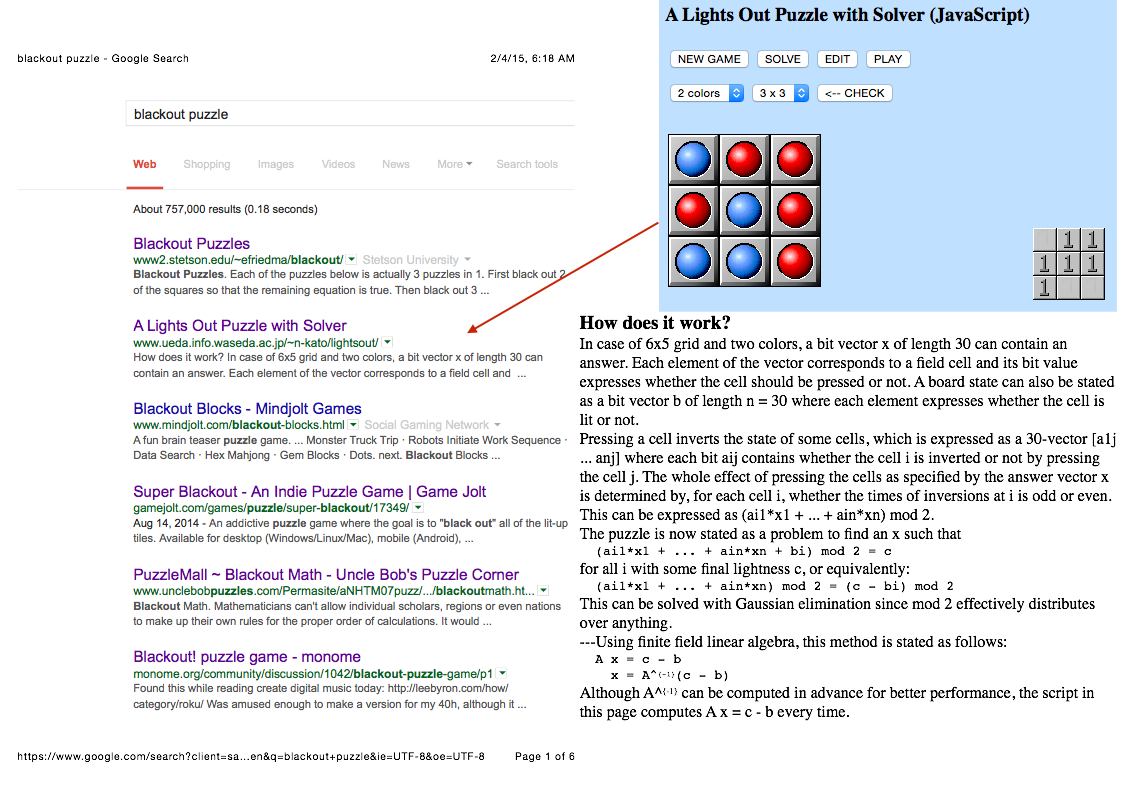
\includegraphics[width=0.95\textwidth]{fg-key-blackp-descr-a}
\vspace*{+2ex}% removes white space for the next row of figures
\end{minipage}
\begin{minipage}{0.49\textwidth}
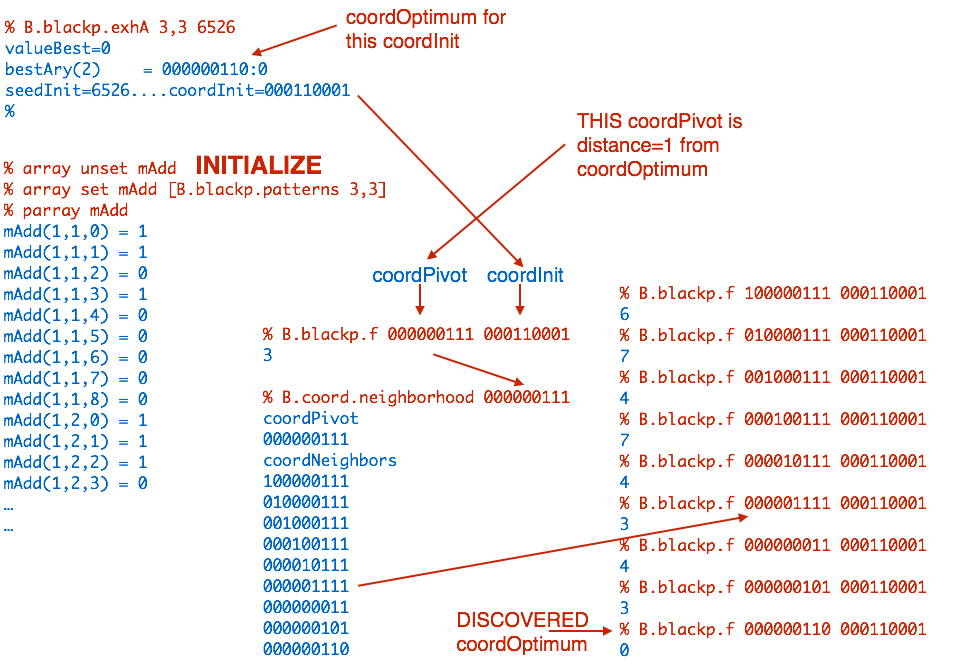
\includegraphics[width=0.95\textwidth]{fg-key-blackp-neighbors}
\vspace*{+2ex}% removes white space for the next row of figures
\end{minipage}
~%
\begin{minipage}{0.49\textwidth}
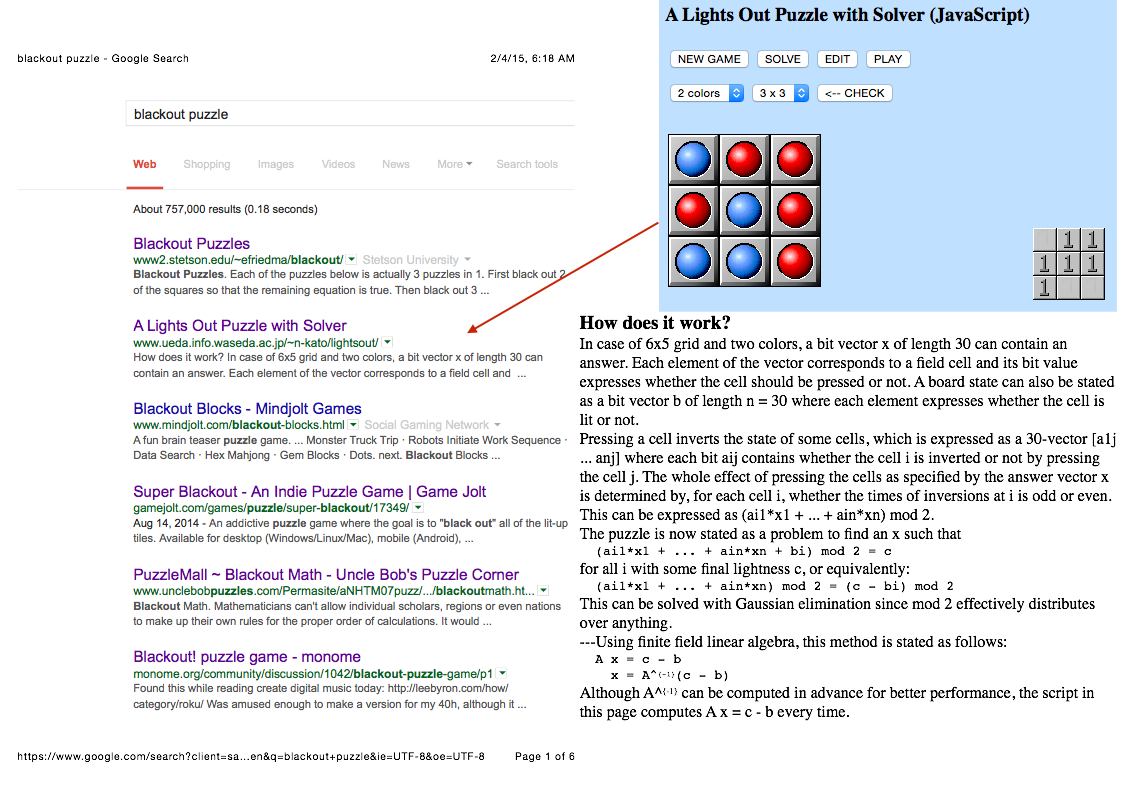
\includegraphics[width=0.95\textwidth]{fg-key-blackp-descr-a}
%\vspace*{+1ex}
\end{minipage}
%
\begin{minipage}{0.49\textwidth}
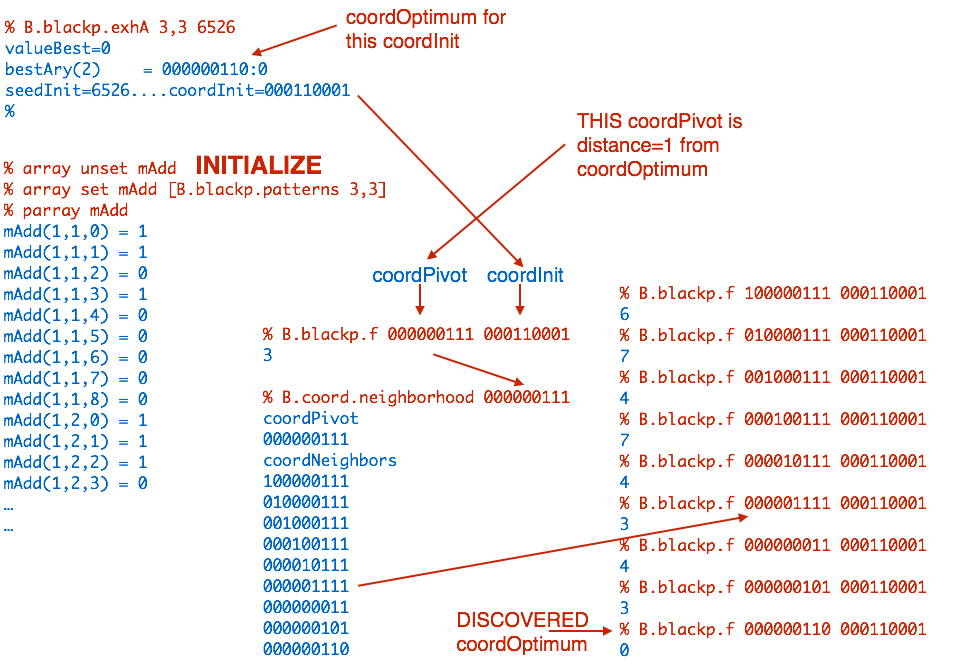
\includegraphics[width=0.95\textwidth]{fg-key-blackp-neighbors}
%\vspace*{-1ex}
\end{minipage}

\caption[From the file fg-key-blackp-wide-4-figures.tex][4ex]
{From the file fg-key-blackp-wide-4-figures.tex {\em borrowed from} {\tt Lib-OPUS2-ebook-CSC499-Sp15-2015-Brglez}.
}
\label{fg-key-blackp-wide-4-figures}
\end{figure*}


\newthought{The file }
fg-key-blackp-wide-4-figures.tex, 
renders Figure~\ref{fg-key-blackp-wide-4-figures}.
\lipsum[4]
\lipsum[4]
